\documentclass[12pt]{standalone}

\RequirePackage{times}
\RequirePackage{amsmath}
\RequirePackage{amssymb}
\RequirePackage[T1]{fontenc}

\usepackage{pgfplots}
\pgfplotsset{compat=1.15}
\usepackage{mathrsfs}
\usetikzlibrary{arrows}
\pagestyle{empty}
\begin{document}
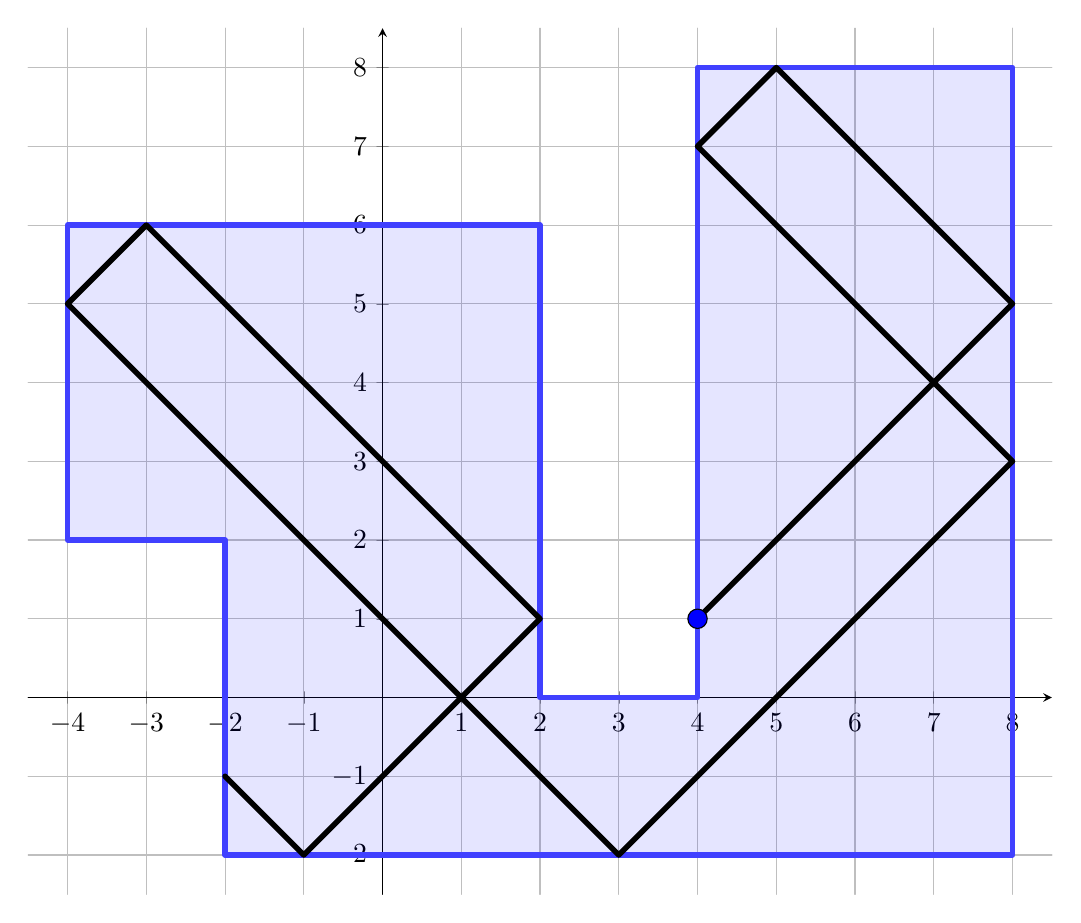
\begin{tikzpicture}[line cap=round,line join=round,>=triangle 45,x=1cm,y=1cm]
    \begin{axis}[
    x=1cm,y=1cm,
    axis lines=middle,
    ymajorgrids=true,
    xmajorgrids=true,
    xmin=-4.5,
    xmax=8.5,
    ymin=-2.5,
    ymax=8.5,
    xtick={-4,-3,...,8},
    ytick={-2,-1,...,8},]
        \draw[line width=2pt,color=blue!75,fill=blue,fill opacity=0.1] (-2,-2) -- (-2,2) -- (-4,2) -- (-4,6) -- (2,6) -- (2,0) -- (4,0) -- (4,8) -- (8,8) -- (8,-2) -- cycle;
        \draw [line width=2pt] (-2,-1)-- (-1,-2)-- (2,1)-- (-3,6)-- (-4,5)-- (3,-2)-- (8,3)-- (4,7)-- (5,8)-- (8,5)-- (4,1);
        \draw [fill=blue] (4,1) circle (3.5pt);
    \end{axis}
\end{tikzpicture}
\end{document}
